

\documentclass{article}

\usepackage[margin=1in]{geometry} 
\usepackage{amsmath,amsthm,amssymb}
\usepackage{esvect}
\usepackage{setspace}
\usepackage{siunitx}
\usepackage{graphicx}
\usepackage{float}
\usepackage{indentfirst}
\usepackage{caption}
\usepackage{listings}
\usepackage{graphics}

\usepackage{amsmath}
\usepackage{algorithm}
\usepackage[noend]{algpseudocode}

\makeatletter
\def\BState{\State\hskip-\ALG@thistlm}
\makeatother



\newcommand{\R}{\mathbb{R}}  
\newcommand{\Z}{\mathbb{Z}}
\newcommand{\N}{\mathbb{N}}
\newcommand{\Q}{\mathbb{Q}}
\newcommand{\C}{\mathbb{C}}

\newenvironment{theorem}[2][Theorem]{\begin{trivlist}
\item[\hskip \labelsep {\bfseries #1}\hskip \labelsep {\bfseries #2.}]}{\end{trivlist}}
\newenvironment{lemma}[2][Lemma]{\begin{trivlist}
\item[\hskip \labelsep {\bfseries #1}\hskip \labelsep {\bfseries #2.}]}{\end{trivlist}}
\newenvironment{exercise}[2][Exercise]{\begin{trivlist}
\item[\hskip \labelsep {\bfseries #1}\hskip \labelsep {\bfseries #2.}]}{\end{trivlist}}
\newenvironment{problem}[2][Problem]{\begin{trivlist}
\item[\hskip \labelsep {\bfseries #1}\hskip \labelsep {\bfseries #2.}]}{\end{trivlist}}
\newenvironment{question}[2][Question]{\begin{trivlist}
\item[\hskip \labelsep {\bfseries #1}\hskip \labelsep {\bfseries #2.}]}{\end{trivlist}}
\newenvironment{corollary}[2][Corollary]{\begin{trivlist}
\item[\hskip \labelsep {\bfseries #1}\hskip \labelsep {\bfseries #2.}]}{\end{trivlist}}

\newenvironment{solution}{\begin{proof}[Solution]}{\end{proof}}

\begin{document}

% ------------------------------------------ %
%                 START HERE                 %
% ------------------------------------------ %

\title{EECS 488 Midterm Report} % Replace X with the appropriate number
\author{Jerome Mao} % Replace "Author's Name" with your name
\maketitle

\setlength{\parindent}{1cm}
\onehalfspacing
\tableofcontents
\newpage

\section{Introduction}
\indent In this project we will develop a smart surveillance camera system, which automatically detects the suspicious approaching the warehouse. It has different modes (the vigilance level). In different levels it will output different media to the local storage or network interface, (e.g., pictures and videos). It will also start a timer when detects suspicious, and will alarm if the owner does not respond to it. The system includes a central host (Raspberry Pi 3) and 8 cameras. Detailed device breakdown will be introduced later.

\section{Event/Mode Switching}
\indent This system has four event/modes; their relationship is stated in [Figure 1]. Event 1 has the lowest alarm level; this mode is set default when no suspicious is detected. Once a suspicious passing by the system will transfer to Event 2, where system will take low resolution pictures on suspicious 2 frames per second. If the suspicious starts to approach the warehouse Event 3 will then be triggered. In which event the same rate of pictures will be taken, but with a higher resolution. Finally, if the suspicious is keeping approaching, the Event 4 will then be triggered, where the system will take movie clips on the target.\newline 
\indent In any event if the suspicious leaves the warehouse, current even will be released and transferred to Event 1.
\begin{figure}[h!]
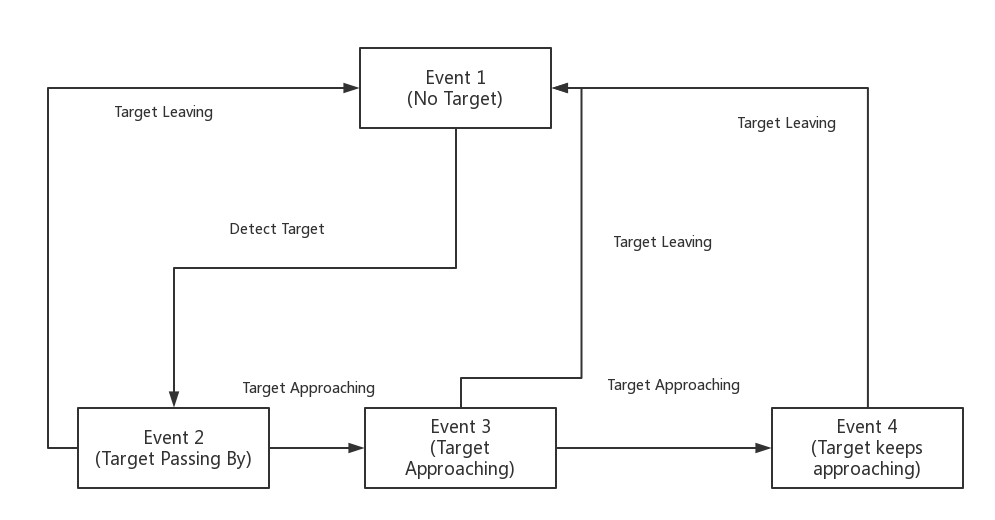
\includegraphics[width=12cm]{EECS488_Flow_Chart.png}
\caption{The logical relationship between four modes in surveillance system}
\end{figure}

\section{Specification}
\indent This section specifies the details in [Event/Mode Switching] section. It also introduces the attributes of the output media. The specification for media and camera operation are separately specified in [Table 1] and [Table 2], accordingly.
\begin{table}[h]

\begin{tabular}{ | l | l | l |}
    \hline
     Name & Technical Specification \\ \hline
     Output Video Format & The output video is MPEG encoded \\ \hline
     Output Video Frame Rate & The output video is 24 fps \\ \hline
     Output Video Resolution & The output video is $1280\times720$ pixels per frame\\ \hline
     Output Picture Format & The output picture is JPEG encoded \\ \hline
     Low Resolution Mode & The output picture is $640\times480$ pixels \\ \hline
     High Resolution Mode & The output picture is $1280\times720$ pixels \\ \hline
\end{tabular}

    \caption{The specification of the output media}
\end{table}

\begin{table}[h]
\begin{tabular}{ | l | l | l |}
    \hline
     Name & Technical Specification \\ \hline
     Alarm Waiting Time & 5 minutes \\ \hline
     Alarm Triggered Level & Event 3 \\ \hline
     Alarm Release Time & Immediately when the mode switches to Event 1 \\ \hline
     Event Lower   Time (From High Event to Event 1) & 5 seconds \\ \hline
     Event Elevate Time (From Low Event to High) & Immediately when condition meets\\ \hline
\end{tabular}

    \caption{The specification of the camera operation}
\end{table}




\section{Software System Design}

\subsection{Introduction and Work Flow}
\indent The software system is split into per camera architecture, which means all 8 cameras share the same design of the software, but runs separately. The process group per camera is specified below in [Figure 2].\newline
\indent The three concurrent processes communicate through queue (for interprocess communication). The queue will transfer two kinds of objects, signals and frames. Signals are integers that indicate the start or end of the work flow. The process that receives signals will forward the signal and get ready for the work, or tear down and recycle the resource allocated. In this project 1 represents start of work and 2 represents the end of work.\newline
\indent Another important use of the queue is to transfer frames. The video capture process keeps sending frames to detector process, and the detector process identifies human faces and forwards (or does nothing accordingly) the tagged frames to the video export process.

\begin{figure}[h!]
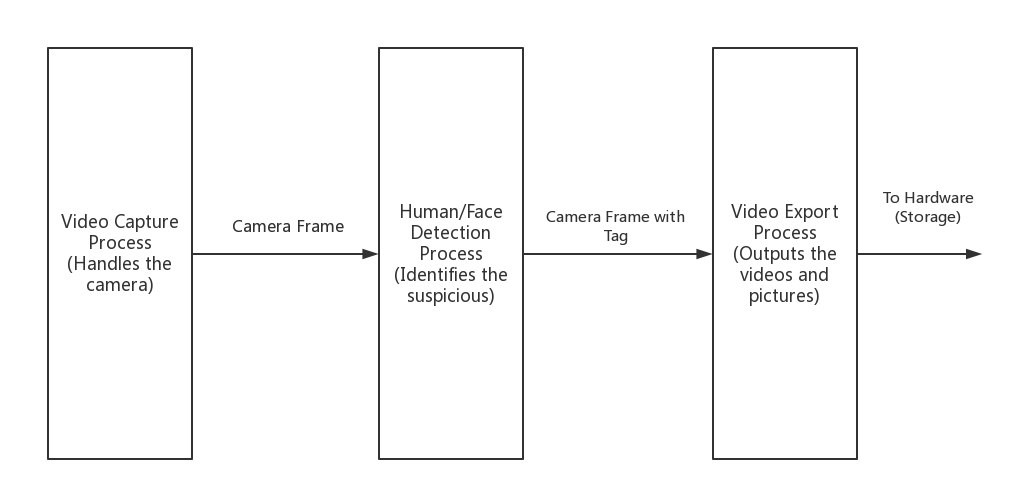
\includegraphics[width=12cm]{EECS488_Sofware_Diagram.png}
\caption{The working flow of three concurrent processes in each camera controller}
\end{figure}

\subsection{Finite State Machine}
\indent To demonstrate the work state for each process, the FSM like graph is provided below in [Figure 3]. This is not strictly a finite state machine, as it contains both conditions and actions. However it is handy to show the life of a single frame on how it is processed from the capture to final export.

\begin{figure}[h!]
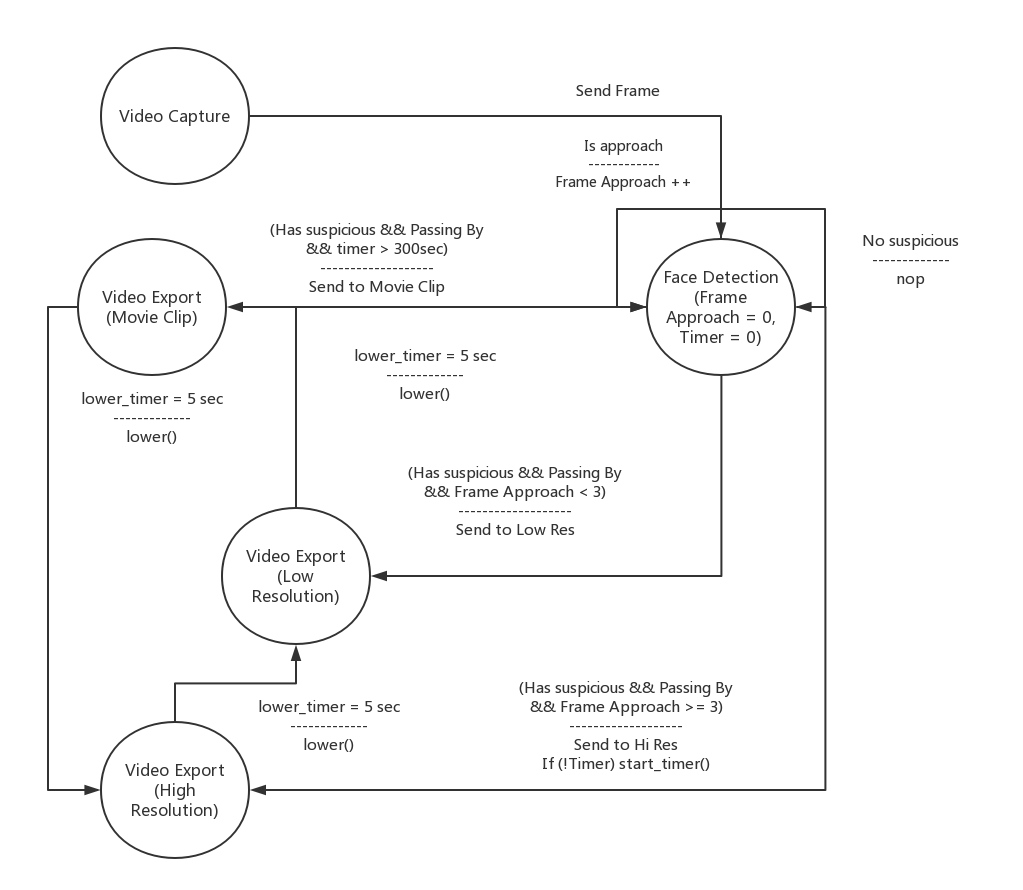
\includegraphics[width=12cm]{EECS488_FSM.png}
\caption{The finite state machine like graph for a single camera handler}
\end{figure}

\indent Please be advised that some arrows are merged together.\newline
\indent From the graph we can see that the detection process is the central dispatcher of each camera instance. The video capture process keeps sending the frames to the human detection process. This process checks whether their is a suspicious, whether the suspicious is approaching, and whether to raise the event level. Then the face detection process sends the frame (or just throw away the frame because it does not include human faces) to the corresponding video export states. Please note that although there are three different video export states in the graph, there is only one process in the real application.

\subsection{User Interface}
\indent This system grants the user some permission to change part of the specification in runtime or before running. These specifications are stated in [Table 3]
\begin{table}[h]
\begin{tabular}{ | l | l | l |}
    \hline
     Name & When to Change & Value Range \\ \hline
     Alarm Silence & Runtime & True or False \\ \hline
     Alarm Waiting Time & Runtime & 2-10 minutes \\ \hline
     Disable Export & Runtime & True or False \\ \hline
     Event 2 Capture Rate & Runtime & 2-7 frame/second \\ \hline
     Event 3 Capture Rate & Runtime & 2-7 frame/second \\ \hline
     Event 4 Video Frame Rate & Before Running & 12, 23.976, 24 fps \\ \hline
     Event 4 Video Resolution & Before Running & $1280\times720$ or $640\times480$ \\ \hline
     
\end{tabular}

    \caption{The specification that can be changed by users}
\end{table}

\subsection{Implementation}
\indent The software system is purely developed with Python 3.X; the multiprocessing related functions are handled by Python multiprocessing standard library, include Process class and multiprocessing.queue.\newline
\indent The image processing functions are depend on OpenCV for Python. Video capture process uses the "VideoCapture" class in OpenCV, but adds a wrapper to it and makes it more easy to use and resource safe. Human Detection process uses "Haar Cascade classifier" in OpenCV, along with a XML file which saves the training data. The video export process uses "VideoWriter" class in OpenCV for video output, and "imsave" function for picture export.

\section{Hardware System}

\subsection{Hardware Modules Involved}
\indent The hardware can also be split into three major sections based on the same functionality as the software. The hardware needed for the three functionalities are listed in [Figure 4].

\begin{figure}[h!]
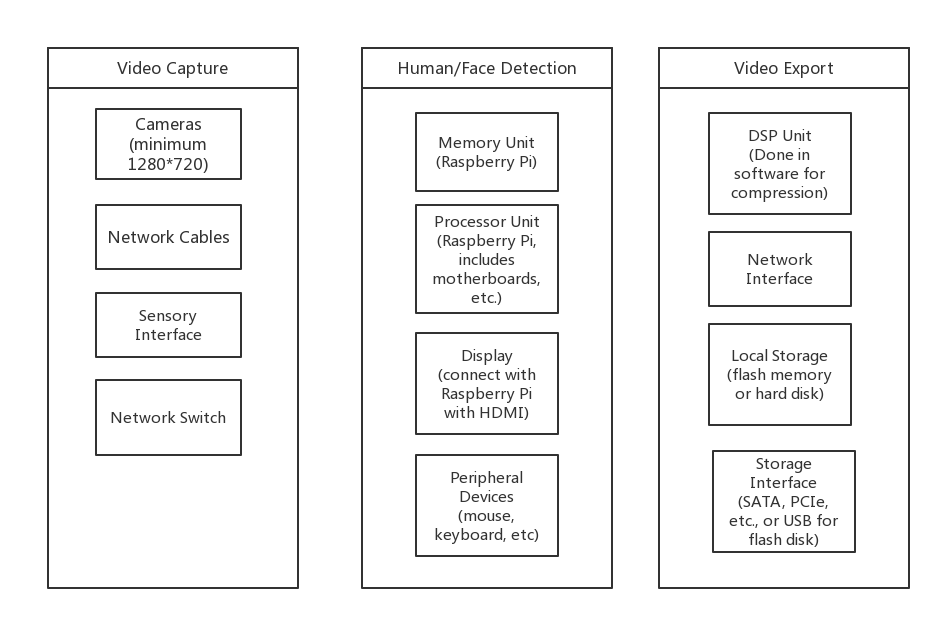
\includegraphics[width=12cm]{EECS488_hardware.png}
\caption{The hardwares needed for each section for the whole system}
\end{figure}
\indent This part needs few clarifications: The video capture can have several either camera with USB 2.0 or 3.0. The minimum requirement is that the camera can provide a stable data stream of $1280\times720$ at the frame rate of 24 fps, as stated in [Specification] section.\newline
\indent The memory unit, processor unit and network interface are in Raspberry Pi 2B. The storage also comes with Raspberry Pi, but it is expandable. In addition, using high resolution camera may need to upgrade the Raspberry Pi to Model 3 B, which has almost the same price as 2B\newline
\indent Raspberry Pi 2B only has one HDMI socket, thus it can only connect to one display.

\subsection{Preliminary Component Cost}
\indent The table below shows a sample assembly and the estimated cost of the system. Please note that it is just a sample, as it uses Raspberry 2B as the host. Model 3B can be another choice with almost the same cost. This system does not include sensory interface, as the SV3C security camera can connect to the network switch. An alternative would be replacing the switch with a router, and using wireless cameras; this improves the mobility of the surveillance system.

\begin{table}[h]

\begin{tabular}{ | l | l | l |}
    \hline
     Name & Unit & Price \\ \hline
     Raspberry Pi Model 2 B & Memory \& Processor & \$70 \\ \hline
     SV3C Ethernet Security Camera $\times8$ & Camera & $\$40\times8=\$320$ \\ \hline
     Dell SE2416HX 23.8" Screen LED-Lit IPS Monitor & Display & \$130 \\ \hline
     Cisco SLM2024T-NA Smart Gigabit Switch SG200-26 & Network Switch & \$250 \\ \hline
     Cat-6 Ethernet Patch Cable $\times9$ & Network Cable & $\$5\times9=\$45$ \\ \hline
     AmazonBasics mouses and keyboard & Peripheral Devices & $\$12+\$7=\$19$ \\ \hline
     Seagate Backup Plus 2TB External Hard Drive & Storage & \$65 \\ \hline\hline
     Total & N/A & \$899 \\ \hline
\end{tabular}

    \caption{The estimated cost of the system}
\end{table}











\end{document}
